\chapter{Details}\label{chap:details}
\section{Path Following and Potential Fields}
While developing our search algorithms in the last lab we realized that doing full $A^*$ searching was not going to be possible in ruby if our discretization was too granular. To alleviate this problem Duane Johnson developed a small library written in C which acted as a module to the rest of our code.  We also simplified the representation of the discretized map for the algorithm to search through.  With these changes we were able to search through maps of 80x80 in approximately 1/10 of a second.  This was fast enough and granular enough for the purpose of finding our way through a maze and deploying a decoy-sniper tactic.
\par
When it came time to follow the solution path returned by Duane's $A^*$ module the immediate thought was to use potential fields along the length of the path.  The potential fields code developed in the first lab already had a PD controller which would suggest velocity and angular velocity based on the current position and angle of the tank.  As the lab progressed we optimized this algorithm to actually look as far ahead as the line segments are parallel so that when driving in a straight line we don't spend much time re-evaluating the path.  We also periodically re-evaluate the search solution which will be important in the future when we are trying to avoid enemy tanks and our world becomes more dynamic.
\par
In addition to the path following optimizations we also `tuned' the relative strength of the fields and their radii so that as we approach the next Potential Field the system will move it to the next location before our arrival.  This helped to avoid uneccesary `braking' and turning.

\section{Schizophrenic Agents}

Multiagent searching often times becomes a process of managing, coordinating and controlling schizophrenic agents.   Each agent is required to play multiple roles, and each of those roles is broken into a series of discrete steps or states.  Each role has a different objective and our task has been to design and coordinate each agent so that they behave in a cohesive manner. We designed our agents such that they used a series of state machines and transitioned from one state to another as each objective was met within the current role. 

\subsection {Agent Design}

We designed the following three state machines: search, decoy, sniper.  The `search' and `decoy' state machines correspond with the roles defined by the lab specification while the `search' machine recycles the common task of ``going to location x, y''.  The states and their corresponding descriptions can be found in tables 3.1, 3.2, and 3.3.  We tried to follow the KISS principle in designing these state machines.  Initially there had been some thought to write higher level intelligence into our agents, but the realization came quickly that, in order to leverage existing potential field code, it would be better to write weak AI agents for now.  The resulting agents are flexible enough for our current goals, and can be augmented for the increased challenges we anticipate in upcoming labs.

The decoy and sniper state machines both rely on using attractive potential fields to move the tank into position.  This was the easiest choice for moving the tanks since the logic to drive a tank based on feedback from potential fields was a solved problem.  This choice proved effective in the end but met some initial problems as some latent bugs had to be rooted out to correct the misbehaving agents.  Once this was accomplished the tanks moved in a fairly predictable and smooth fashion.

\begin{table}[ht]
	\label{sm-smart}
	\caption{State Machine - Smart}
	\begin{center}
		\begin{tabular}{ | p{1.5in} | p{3.5in} |}
		  \hline
			\bf{State} & \bf{Description} \\
			\hline
			smart & Sets the goal for the tank to the exit point of the maze and moves the tank through the maze \\
			\hline
			look\textunderscore for\textunderscore enemy\textunderscore flag & Retrieves the enemy flag \\
			\hline
			return\textunderscore home & Sets the goal to the home, generates a search path and returns to home \\
		  \hline
		\end{tabular}
	\end{center}
\end{table}

\begin{table}[ht]
	\label{sm-decoy}
	\caption{State Machine - Decoy}
	\begin{center}
		\begin{tabular}{ | p{1.5in} | p{3.5in} |}
		  \hline
				\bf{State} & \bf{Description} \\ \hline
				move\textunderscore to\textunderscore start & Sets the destination to the decoy starting position and moves the tank to that point \\ \hline
				move\textunderscore to\textunderscore goal  & Sets the destination to the opposing end of the line and moves the tank to that point \\
		  \hline
		\end{tabular}
	\end{center}
\end{table}

\begin{table}[ht]
	\label{sm-sniper}
	\caption{State Machine - Sniper}
	\begin{center}
		\begin{tabular}{ | p{1.5in} | p{3.5in} |}
		  \hline
				\bf{State} 			& \bf{Description} \\ \hline
				move\textunderscore to\textunderscore start 	& Sets the destination to the sniper starting position and moves the tank to that point \\ \hline
				move\textunderscore to\textunderscore attack  & Sets the destination to the attack position and moves the tank to that point \\ \hline
				attack  				& Snipes the enemy tank(s). \\
		  \hline
		\end{tabular}
	\end{center}
\end{table}

\section{Agent Behavior}

In order to map out the paths to their respective destinations, each agent is initially set to a search state which we labeled ``smart''.  From there, the state transitions bifurcate for each tank---based on the tank ID, it takes on its respective role and continues through the following agent states.

\begin{figure}\label{fig:search}
\begin{center}
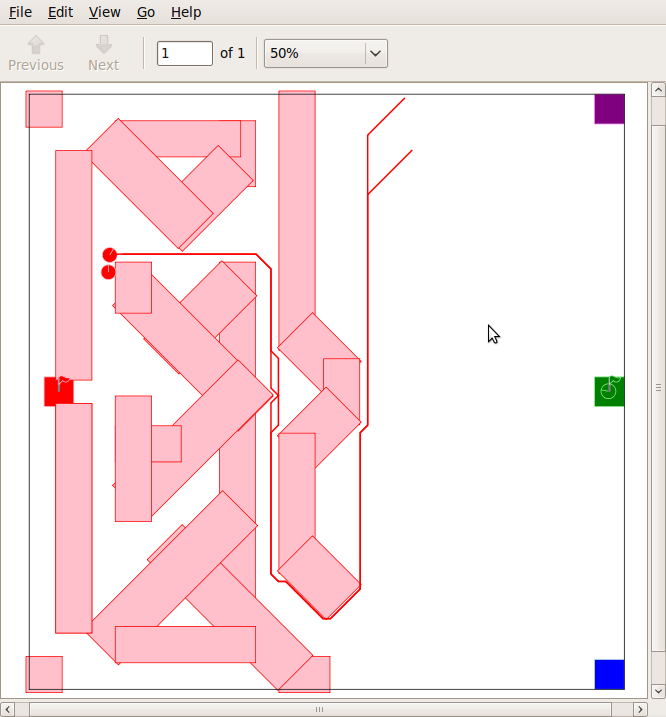
\includegraphics[width=\textwidth]{01paths.png}
\caption{Red agents search out a path to their destinations using the \emph{smart} state.}
\end{center}
\end{figure}

\subsection{Decoy}

The key to meeting the objective of this lab is to ensure that the decoy agent stays closer to the enemy tank as well as keeps from getting shot.  With those two objectives in mind we designed the decoy agent to travel back and forth in a straight line between two ends of the field while maintaing a x-distance of roughly 270 meters.  Therefore we created two states, one to drive us to the starting point (\emph{move\textunderscore to\textunderscore start}) and the second to drive us to the opposite point (\emph{move\textunderscore to\textunderscore goal}).  If an enemy tank is still alive, our tank would move back to the starting point and repeat the cycle.  If all enemy tanks are destroyed, however, then the decoy tank would proceed back to the base by setting the goal to `home base' and switching to the \emph{smart} state machine.

\begin{figure}\label{fig:decoy}
\begin{center}
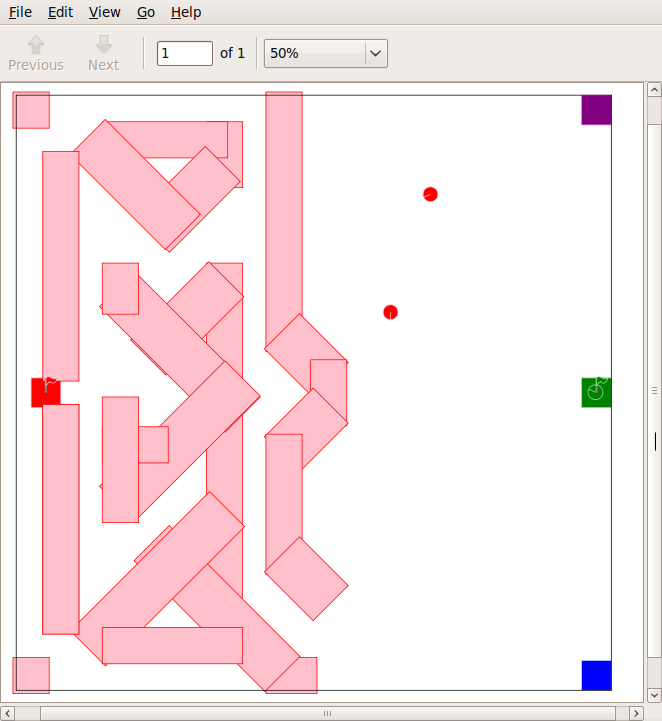
\includegraphics[width=\textwidth]{04decoy.png}
\caption{The sniper agent moves into place (top) and the decoy agent begins its movements back and forth (bottom).}
\end{center}
\end{figure}

\subsection{Sniper}

The sniper agent is designed to move into an initial starting position just outside of the enemy tanks' firing range.  The agent polls periodically to see when the distance between the decoy agent and the enemy tank is smaller than between the sniper and the enemy tank.  When the sniper detects that the decoy is closer, the sniper transitions from \emph{move\textunderscore to\textunderscore start} to \emph{move\textunderscore to\textunderscore attack}.  At this point the sniper moves approximately 5 meters inside of the enemy tanks firing position.  Once the tank has arrived into position it transitions to \emph{attack}.  While in attack mode, the tank stops its speed, turns into position and once the proper angle is set, fires a shot, thus destroying the enemy tank.

\begin{figure}\label{fig:kill}
\begin{center}
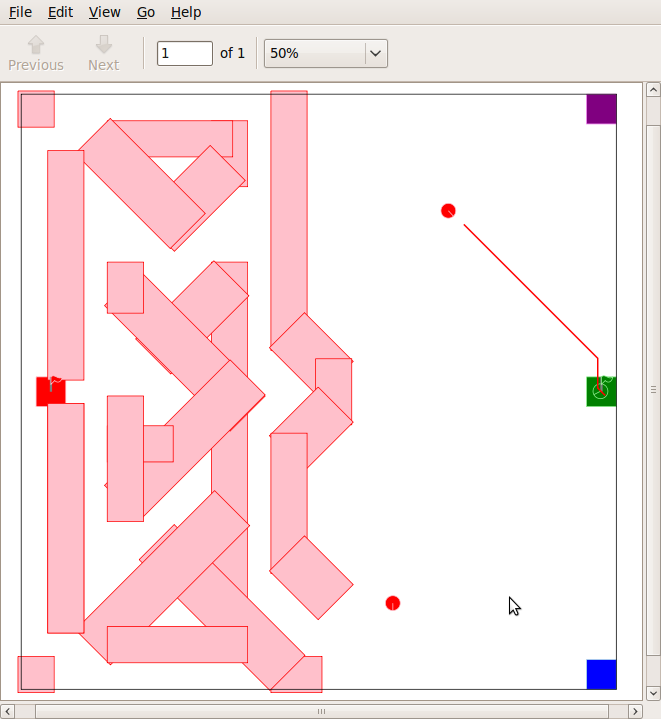
\includegraphics[width=\textwidth]{05kill.png}
\caption{After killing the enemy tank, the sniper agent plots a path to the green flag.}
\end{center}
\end{figure}

\begin{figure}\label{fig:capture}
\begin{center}
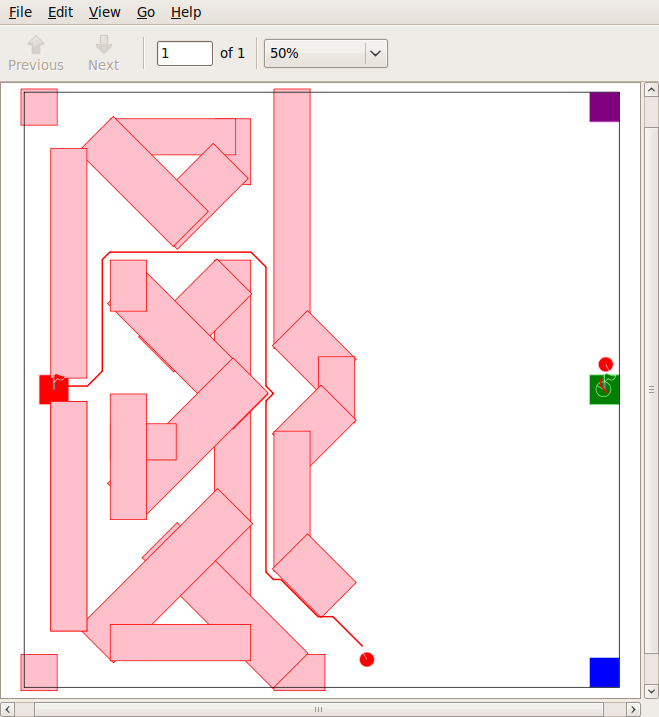
\includegraphics[width=\textwidth]{06capture.png}
\caption{The decoy agent returns to home base while the sniper agent picks up the enemy flag.}
\end{center}
\end{figure}

\subsection{Looking to the Future}

In completing this lab a few shortcuts were made which will need to be addressed in future labs.  We relied on the fact that the map orientation (i.e. location of the bases, enemy tank locations, and clear location of the world) were in fixed locations.  By making these simplifying assumptions we saved ourselves from writing a bit of code which would have to map out the best path for the decoy, the ideal starting position for the sniper and the ideal sniping position.  These simplifications will obviously have to be addressed if our agents are to be successful in more mobile enemy tanks.

There is still some room for correction in the controlling of our tanks via potential fields and we would probably benefit by adding in a PD controller to dampen our movement since there are times when the tank does not slow down or turn in a smooth fashion.  Our tanks at times seem to favor turning in a certain direction, which points to a bug in our code.  By fixing this I believe most, if not all, of our agents driving problems would be solved.

We made another simplification by not coordinating the efforts between the sniper and the decoy, but instead relying on the timing and initial positioning to keep our sniper safe.  However when faced with more tanks, the sniper does not currently move in closer to engage multiple targets if they are not all reachable when it moves into attack mode.

\section{Tests with Another Group}
\subsection{Our Tests}
We ran the tests for our implementation on the \emph{astar.bzw} map from the lab website. Our tests went well with the exception of the return trip to our base after capturing the flag.  This is the one odd behavior for which no solution has yet been found.
\par
\begin{figure}\label{fig:stuck}
\begin{center}
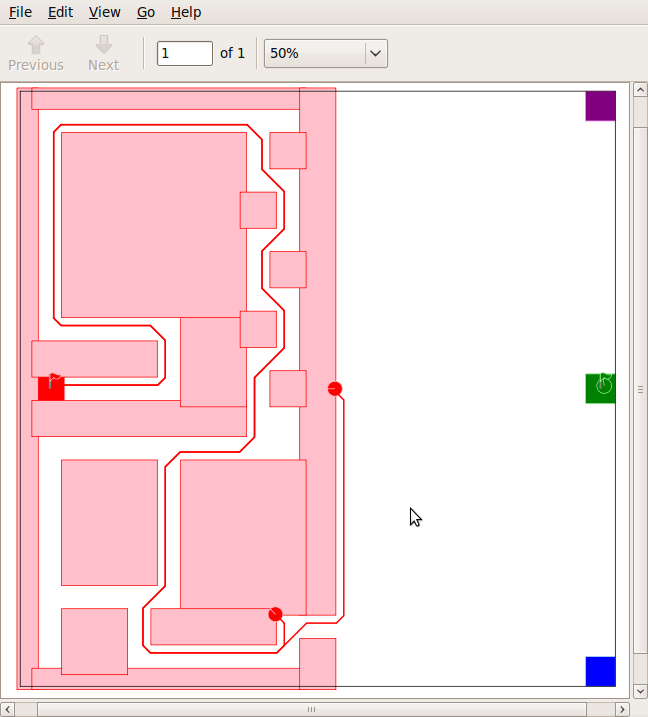
\includegraphics[width=\textwidth]{07re-evaluate-path.png}
\caption{Getting stuck at the wall on the way home. Re-evaluated path shown as red line to red base.}
\end{center}
\end{figure}

While demonstrating the code we ran into two difficulties.  The first difficulty came when the sniper tank missed picking up the flag and then proceeded to try to return to base.  The second came after we fixed the code and reran the agents.  After the agent picked up the flag it used the wrong field for a while until the agent realized that it's search.  Once the search path was re-evaluated it returned to home base successfully.

While our code demonstratably has some fragile edges, it appears from having observed several other teams code that ours is not alone, however, to its credit it did manage to satisfy the requirements for the lab.

\subsection{Michael Hansen and Daniel Nelson}
We ran our tests with another group from class which consisted of:
\begin{itemize}
    \item{Michael Hansen}
    \item{Daniel Nelson}
\end{itemize}
What was interesting about watching the other team pass off was that they had a few problems in their implementation, but they were in no way related to the problems we encountered.  The main problem the other team had was that the decoy would get killed as it went into its decoy mode.  They had to change the timing of their agents to avoid this, but in the end they successfully completed the challenge.

\subsection{Kendall Clement et. al.}
In addition to Hansen and Nelson's group, we watched Kendell demonstrate his code.  It was quite entertaining because while his team had already passed off his bot was defeated a couple of times before it finally worked.  When the bot was able to finally successfully kill the agent, it grabbed the flag and eventually made its way back to the base; however it skirted the edge of the base and as a result the system did not register the capture---presumably because his tank never entered the circle inside of the base.

The other interesting points of watching his demonstration was to see how his tank seemed to bounce between walls and moved from one wall to another (i.e. a side to side action), in addition it ran into walls when it needed to turn more tightly.  Other than that I did think that their overall approach for running the decoy was a bit better than ours and it completes in a faster manner than ours (in the case where it succeeds, at least).
